\subsection{Đề 3}
\Opensolutionfile{ans}[ans/ans-CTST_1-OTGK1_De3-LC]
\caulc
\begin{ex} %[1D1N1-2]
	Cho góc lượng giác $(OA,OB)$ có số đo bằng $\dfrac{\pi}{6}$. Hỏi trong các số đo góc sau, số đo nào là số đo của một góc lượng giác có cùng tia đầu, tia cuối với góc lượng giác $(OA,OB)$?
	\choice
	{$\dfrac{-49\pi}{6}$}
	{$-\dfrac{7\pi}{6}$}
	{$\dfrac{7\pi}{6}$}
	{\True $\dfrac{49\pi}{6}$}
	\loigiai{
		Áp dụng kiến thức: Số đo của các góc lượng giác có chung tia đầu, tia cuối sai khác nhau một bội nguyên của $2\pi$.\\
		Ta thấy $\dfrac{49\pi}{6}-\dfrac{\pi}{6}=4\cdot2\pi$.}
\end{ex}
\begin{ex}%[1D1N2-3]
	Giá trị biểu thức $C=\cos \dfrac{\pi }{6}+\sin \dfrac{\pi }{2}+\tan \pi +\cot \dfrac{\pi }{4}$ bằng
	\choice
	{$C=\dfrac{4-\sqrt{3}}{2}$}
	{$C=\dfrac{6+\sqrt{3}}{2}$}
	{\True $C=\dfrac{4+\sqrt{3}}{2}$}
	{$C\approx 74{,}03$}
	\loigiai{
		Ta có $C=\cos \dfrac{\pi}{6}+\sin \dfrac{\pi}{2}+\tan \pi +\cot \dfrac{\pi }{4}=\dfrac{\sqrt{3}}{2}+1+0+1=\dfrac{4+\sqrt{3}}{2}$.}
\end{ex}
\begin{ex}%[1D1N3-2]
	Cho $a+b=\dfrac{\pi}{3}$. Giá trị biểu thức $T=\cos a\cos b-\sin a\sin b$ bằng
	\choice
	{$1$}
	{$-1$}
	{$\dfrac{\sqrt{3}}{2}$}
	{\True $\dfrac{1}{2}$}
	\loigiai{
		Ta có $T=\cos a\cos b-\sin a\sin b=\cos \left( a+b \right)=\cos \dfrac{\pi }{3}=\dfrac{1}{2}$.}
\end{ex}
\begin{ex}%[1D1N2-4]
	Tính giá trị của $\cos \left[ \dfrac{\pi }{3}+\left( 2k+1 \right)\pi \right]$ với $k$ là số nguyên.
	\choice
	{$\cos \left[ \dfrac{\pi }{3}+\left( 2k+1 \right)\pi \right]=-\dfrac{\sqrt{3}}{2}$}
	{$\cos \left[ \dfrac{\pi }{3}+\left( 2k+1 \right)\pi \right]=\dfrac{1}{2}$}
	{\True $\cos \left[ \dfrac{\pi }{3}+\left( 2k+1 \right)\pi \right]=-\dfrac{1}{2}$}
	{$\cos \left[ \dfrac{\pi }{3}+\left( 2k+1 \right)\pi \right]=\dfrac{\sqrt{3}}{2}$}
	\loigiai{
		Ta có $\cos \left[ \dfrac{\pi }{3}+\left( 2k+1 \right)\pi \right]=\cos \left( \dfrac{\pi }{3}+\pi +k2\pi \right)=\cos \left( \dfrac{\pi }{3}+\pi \right)=-\cos \dfrac{\pi }{3}=-\dfrac{1}{2}.$}
\end{ex}
\begin{ex}%[1D1N4-4]
	Trong các hàm số sau, hàm số nào là hàm số chẵn?
	\choice
	{$y=\sin x$}
	{\True $y=\cos x$}
	{$y=\tan x$}
	{$y=\cot x$}
	\loigiai{
		Nhắc lại kiến thức cơ bản:\\
		Hàm số $y=\sin x$ là hàm số lẻ.\\
		Hàm số $y=\cos x$ là hàm số chẵn.\\
		Hàm số $y=\tan x$ là hàm số lẻ.\\
		Hàm số $y=\cot x$ là hàm số lẻ.
		}
\end{ex}
\begin{ex}%[1D1N4-5]
	Hãy chỉ ra hàm số tuần hoàn trong các hàm số sau.
	\choice
	{$y=x\sin x$}
	{\True $y=\sin 3x$}
	{$y=x-\sin x$}
	{$y=\dfrac{x}{2+\sin x}$}
	\loigiai{
		Hàm số $y=\sin u(x)$ là hàm tuần hoàn. Vậy $y=\sin 3x$ là hàm tuần hoàn.}
\end{ex}
\begin{ex}%[1D1N4-6]
	Tìm tập giá trị của hàm số sau $y=\dfrac{2023}{\sin x}$.
	\choice
	{$T=\mathbb{R}\setminus \{0\}$}
	{$T=[-2023;2023]$}
	{$T=\mathbb{R}$}
	{\True $T=(-\infty ;-2023]\cup [2023;+\infty)$}
	\loigiai{
		Ta có $-1\le \sin x\le 1\Rightarrow \dfrac{1}{\sin x}\le -1$ hoặc $\dfrac{1}{\sin x}\ge 1$.\\
		Suy ra $\dfrac{2023}{\sin x}\le -2023$ hoặc $\dfrac{2023}{\sin x}\ge 2023$.\\
		Vậy $T=(-\infty;-2023]\cup [2023;+\infty)$.}
\end{ex}
\begin{ex}%[1D2N1-5]
	Cho dãy số $({u_n})$ với $u_n=2n-1$. Dãy số $(u_n)$ là dãy số
	\choice
	{Bị chặn trên bởi $1$}
	{Giảm}
	{Bị chặn dưới bởi $2$}
	{\True Tăng}
	\loigiai{
		Với $\forall n\in \mathbb{N}^{*}$ ta có $u_{n+1}-u_n=2(n+1)-1-(2n-1)=2>0$ nên $u_{n+1}>u_n$.\\
		 Vậy dãy số $(u_n)$ tăng.}
\end{ex}
\begin{ex}%[1D2N1-4]
	Cho dãy số $(u_n)$ có $u_n=\sin \dfrac{\pi}{n}$. Chọn khẳng định đúng trong các khẳng định sau đây.
	\choice
	{\True Dãy số $(u_n)$ bị chặn}
	{Dãy số $(u_n)$ tăng}
	{Dãy số $(u_n)$ giảm}
	{Dãy số $(u_n)$ không bị chặn}
	\loigiai{
		Do $-1\le \sin \dfrac{\pi}{n}\le 1$ nên dãy số $(u_n)$ bị chặn.}
\end{ex}
\begin{ex}%[1D2H2-2]
	Dãy số nào sau đây là một cấp số cộng?
	\choice
	{\True $(u_n)\colon \heva{ 
			&u_1=2 \\
			&{u_{n+1}}=u_n+3,\,\,\forall n\ge 1}$}
	{$(u_n)\colon \heva{ 
			&u_1=3 \\
			&{u_{n+1}}=2u_n-4,\,\,\forall n\ge 1}$}
	{$(u_n)\colon 1$; $-3$; $6$; $7$; $15$; $\ldots$}
	{$(u_n)\colon -1$; $1$; $-1$; $1$; $-1$; $\ldots$}
	\loigiai{
		Dãy số $(u_n)\colon \heva{ 
			&u_1=2 \\
			&{u_{n+1}}=u_n+3,\,\,\forall n\ge 1 } $ thỏa $u_{n+1}-u_n=3$ với mọi $n\ge 1$ nên là cấp số cộng.}
\end{ex}
\begin{ex}%[1D2N2-2]
	Cho cấp số cộng $(u_n)$ có $u_2=8$, $u_5=17$. Công sai $d$ bằng
	\choice
	{$d=-3$}
	{$d=-5$}
	{\True $d=3$}
	{$d=5$}
	\loigiai{
		Ta có $ \heva{ 
			&u_2=8 \\
			&u_5=17 } \Leftrightarrow \heva{ 
			&u_1+d=8\\
			&u_1+4d=17 } \Leftrightarrow \heva{ 
			&u_1=5 \\
			&d=3.}$\\
		Vậy công sai $d=3$.}
\end{ex}
\begin{ex}%[1D2N3-2]
	Trong các dãy số $(u_n)$ sau đây, dãy số nào là cấp số nhân?
	\choice
	{$u_n=(-1)^n\cdot n$}
	{$u_n=n^2$}
	{\True $u_n=2^n$}
	{$u_n=\dfrac{n}{3^n}$}
	\loigiai{
		Lập tỉ số $\dfrac{u_{n+1}}{u_n}$.
		\begin{itemize}
		\item $\dfrac{u_{n+1}}{u_n}=\dfrac{(-1)^{n+1}\cdot (n+1)}{(-1)^n\cdot n}=-\dfrac{n+1}{n}\Rightarrow (u_n)$ không phải cấp số nhân.\\
		\item $\dfrac{u_{n+1}}{u_n}=\dfrac{(n+1)^2}{n^2}\Rightarrow (u_n)$ không phải là cấp số nhân.\\
		\item $\dfrac{u_{n+1}}{u_n}=\dfrac{2^{n+1}}{2^n}=2\Rightarrow u_{n+1}=2u_n\Rightarrow (u_n)$ là cấp số nhân có công bội bằng $2$.\\
		\item $\dfrac{u_{n+1}}{u_n}=\dfrac{n+1}{3n}\Rightarrow (u_n)$ không phải là cấp số nhân.
		\end{itemize}
	}
\end{ex}
\Closesolutionfile{ans}
\indapan{6}{ans/ans-CTST_1-OTGK1_De3-LC}
%-------------------------------------------
\Opensolutionfile{ans}[ans/ans-CTST_1-OTGK1_De3-DS]
\cauds
\begin{ex}%[1D2H3-5]
	Cho cấp số nhân $(u_n)$ có $u_1=\dfrac{1}{2},q=-2$.
	\choiceTF
	{\True Số hạng thứ 3 là $u_3=2$}
	{Tổng của 5 số hạng đầu là của cấp số nhân là $\dfrac{85}{4}$}
	{Cấp số nhân đã cho là một dãy số tăng}
	{\True Số $-1024$ là số hạng thứ 12 của cấp số nhân}
	\loigiai{
		\begin{itemchoice}
	\itemch Đúng. Vì $u_3=u_1\cdot q^2=\dfrac{1}{2}\cdot (-2)^2=2$.\\
	\itemch Sai. Vì tổng của $5$ số hạng đầu là $S_5=u_1\dfrac{1-q^5}{1-q}=\dfrac{1}{2}\cdot \dfrac{1-(-2)^5}{1-(-2)}=\dfrac{11}{2}$.\\
		\itemch Sai. Vì $u_1=\dfrac{1}{2}$, $u_2=-1$, $u_3=2$.\\
		\itemch Đúng. Ta có $u_n=u_1\cdot q^{n-1}=-1024$.\\
		Nên $u_1\cdot q^{n-1}\Leftrightarrow \dfrac{1}{2}\cdot(-2 )^{n-1}=-1024\Leftrightarrow (-2)^{n-1}=(-2)^{11}\Leftrightarrow n=12$.
	\end{itemchoice}}
\end{ex}
\begin{ex}%[1D1V5-5]
	Cho phương trình $\cos^2\left(2x+\dfrac{\pi}{4}\right)+\cos^2\left(x+\dfrac{\pi}{2}\right)=1$.
	\choiceTF
	{\True Phương trình đã cho được viết lại như sau $\sin^2\left(2x+\dfrac{\pi}{4}\right)=\cos^2\left(x+\dfrac{\pi}{2}\right)$}
	{\True Ta có $\cos\left(2x+\pi\right)=-\cos2x$}
	{\True Phương trình đã cho đưa về dạng $\cos\left(4x+\dfrac{\pi}{2}\right)=\cos2x$}
	{Nghiệm của phương trình đã cho là $x=-\dfrac{\pi}{4}+k\pi$ và $x=\dfrac{\pi}{12}+k\dfrac{\pi}{3}~\left(k\in \mathbb{Z}\right)$}
	\loigiai{
			\begin{itemchoice}
			\itemch \textbf{Đúng}.
			Ta có
			\begin{eqnarray*}
				&&\cos^2\left(2x+\dfrac{\pi}{4}\right)+\cos^2\left(x+\dfrac{\pi}{2}\right)=1\\
				&\Leftrightarrow & \sin^2\left(2x+\dfrac{\pi}{4}\right)=\cos^2\left(x+\dfrac{\pi}{2}\right)
			\end{eqnarray*}
			\itemch \textbf{Đúng}. Ta có $\cos\left(2x+\pi\right)=-\cos2x$
			\itemch \textbf{Đúng}.
			Ta có
			\begin{eqnarray*}
				&&\cos^2\left(2x+\dfrac{\pi}{4}\right)+\cos^2\left(x+\dfrac{\pi}{2}\right)=1\\
				&\Leftrightarrow & \sin^2\left(2x+\dfrac{\pi}{4}\right)=\cos^2\left(x+\dfrac{\pi}{2}\right)\\
				&\Leftrightarrow & \dfrac{1-\cos\left(4x+\frac{\pi}{2}\right)}{2}=\dfrac{1+\cos\left(2x+\pi\right)}{2}\\
				&\Leftrightarrow & -\cos\left(4x+\dfrac{\pi}{2}\right)=\cos\left(2x+\pi\right)\\
				&\Leftrightarrow & -\cos\left(4x+\dfrac{\pi}{2}\right)=-\cos2x\\
				&\Leftrightarrow & \cos\left(4x+\dfrac{\pi}{2}\right)=\cos2x
			\end{eqnarray*}
			\itemch \textbf{Sai}.
				Ta có
				\begin{eqnarray*}
					&&\cos^2\left(2x+\dfrac{\pi}{4}\right)+\cos^2\left(x+\dfrac{\pi}{2}\right)=1\\
					&\Leftrightarrow & \sin^2\left(2x+\dfrac{\pi}{4}\right)=\cos^2\left(x+\dfrac{\pi}{2}\right)\\
					&\Leftrightarrow & \dfrac{1-\cos\left(4x+\frac{\pi}{2}\right)}{2}=\dfrac{1+\cos\left(2x+\pi\right)}{2}\\
					&\Leftrightarrow & -\cos\left(4x+\dfrac{\pi}{2}\right)=\cos\left(2x+\pi\right)\\
					&\Leftrightarrow & -\cos\left(4x+\dfrac{\pi}{2}\right)=-\cos2x\\
					&\Leftrightarrow & \cos\left(4x+\dfrac{\pi}{2}\right)=\cos2x
				\end{eqnarray*}
				$$\Leftrightarrow\hoac{&4x+\dfrac{\pi}{2}=2x+k2\pi\\&4x+\dfrac{\pi}{2}=-2x+k2\pi}\Leftrightarrow\hoac{&x=-\dfrac{\pi}{4}+k\pi\\&x=-\dfrac{\pi}{12}+k\dfrac{\pi}{3}}~(k\in \mathbb{Z}).$$
			\end{itemchoice}
	}
\end{ex}
\begin{ex}%[1D2H1-5]
	Cho dãy số $(u_n)$ biết $u_n=2^n+1$. Khi đó
	\choiceTF
	{\True Số hạng thứ $6$ của dãy số là 65}
	{Số hạng thứ $n+2$ của dãy số là $u_{n+2}=2\cdot2^n$}
	{\True Dãy số $(u_n)$ là một dãy số tăng}
	{Dãy số $(u_n)$ là dãy số bị chặn}
	\loigiai{
		\begin{itemchoice}
			\itemch Đúng. Ta có $u_6=2^6+1=65$.
			\itemch Sai. Ta có $ u_n=2^n\Rightarrow u_{n+2}=2^{n+2}+1=4\cdot2^n+1$.
			\itemch Đúng. Ta có $u_{n+1}-u_n=2^{n+1}+1-2^n-1=2\cdot2^n-2^n=2^n>0$, $\forall n\in \mathbb{N}^*$. Do đó dãy số $(u_n)$ là một dãy số tăng.
			\itemch Sai. Vì dãy số $(u_n)$ không bị chặn trên nên dãy số không bị chặn.
		\end{itemchoice}
	}
\end{ex}
\begin{ex}%[1C4H1-6]
	Trong mặt phẳng $(P)$, cho hình bình hành $ABCD$ tâm $O$, ngoài mặt phẳng $(P)$ cho một điểm $S$. 
	\choiceTF
	{Điểm $C$ là một điểm chung của hai mặt phẳng $(SAB)$ và $(SCD)$}
	{\True Giao tuyến của hai mặt phẳng $(SCB)$ và $(SCD)$ là đường thẳng $SC$}
	{\True Giao điểm của mặt phẳng $(SAC)$ với đường thẳng $BD$ là điểm $O$}
	{Giao điểm của đường thẳng $BC$ với mặt phẳng $(SBD)$ là điểm $C$}
	\loigiai{
		\begin{center}
			\begin{tikzpicture}[scale=1, font=\footnotesize, line join=round, line cap=round, >=stealth, blue,thick]
			\def\bc{4} % cạnh BC
			\def\ba{2} % cạnh BA
			\def\h{4} % đường cao
			\def\gocB{35} % góc B của đáy
			\coordinate (M) at (-1.5,-.5);
			\coordinate (N) at (50:2.5);
			\coordinate (Q) at (5,-.5);
			\coordinate (P) at ($(Q)-(M)+(N)$);
			\fill[cyan!20!](M)--(N)--(P)--(Q)--cycle;
			\coordinate[label=below left:$D$] (D) at (0,0);
			\coordinate[label=above left:$A$] (A) at (\gocB:\ba);
			\coordinate[label=below:$C$] (C) at (\bc,0);
			\coordinate[label=above right:$B$] (B) at ($(C)-(D)+(A)$);
			\path 
			(intersection of A--C and B--D) coordinate (O);
			\node at (O) [below]{$O$};
			\coordinate [label=above:$S$](S) at ($(O)+(0,4)$);
			\draw (S)--(D)--(C)--(B)--cycle;
			\draw[dashed,thin] (A)--(C)--(S) (B)--(D) (A)--(S)--(O) (D)--(A)--(B);
			\draw pic["$P$", draw=black, angle eccentricity=.7, angle radius=1cm]	{angle=Q--M--N}; 
			\foreach \i in {A,B,C,D,O,S} \fill[black] (\i) circle (1pt);
		\end{tikzpicture}
	\end{center}
	\begin{itemchoice}
				\itemch Sai. Điểm $C$ không là một điểm chung của hai mặt phẳng $ (SAB)$ và $(SCD)$ vì điểm $C$ không không thuộc mặt phẳng $(SAB)$
				\itemch Đúng. Vì $S$ và $C$ cùng thuộc hai mặt phẳng $(SCB)$ và $ (SCD)$ nên giao tuyến của hai mặt phẳng $(SCB)$ và $(SCD)$ là đường thẳng $SC$.
				\itemch Đúng. Khi đó vì $O$ thuộc mặt phẳng $(SAC)$ nên điểm $O$ là giao điểm của mặt phẳng $(SAC)$ với đường thẳng $BD$.
				\itemch Sai. Vì giao điểm của đường thẳng $BC$ với mặt phẳng $(SBD)$ là điểm $B$.
					\end{itemchoice}
	
	}	
\end{ex}
\Closesolutionfile{ans}
\indapan{3}{ans/ans-CTST_1-OTGK1_De3-DS}
%-------------------------------------------
\Opensolutionfile{ans}[ans/ans-CTST_1-OTGK1_De3-KQ]
\caukq
\begin{ex}%[1D2V1-5]
	Cho dãy số $(u_n)$, biết $u_n=n+\dfrac{1}{n}$. Tìm $m$ để dãy số $(u_n)$ bị chặn dưới bởi $m$.
	\shortans{$2$}
	\loigiai{
		Xét $u_n=n+\dfrac{1}{n}\ge 2\sqrt{n\cdot\dfrac{1}{n}}=2$. (Áp dụng BĐT Côsi)}
\end{ex}
\begin{ex}%[1D2V3-8]
	\immini[thm]{Cho hình vuông $C_1$ có cạnh bằng $4$. Người ta chia mỗi cạnh của hình vuông thành bốn phần bằng nhau và nối các điểm chia một cách thích hợp để có hình vuông $C_2$ như hình vẽ bên.
	Từ hình vuông $C_2$ lại làm tiếp như trên để nhận được hình vuông $C_3$,\ldots. Tiếp tục quá trình trên, ta nhận được dãy các hình vuông $C_1,\,C_2,\,C_3,\ldots,C_n,\ldots$. Gọi $a_n$ là độ dài của cạnh hình vuông $C_n$. Tính tổng diện tích của các hình vuông (kết quả làm tròn đến hàng phần chục).}
	{
	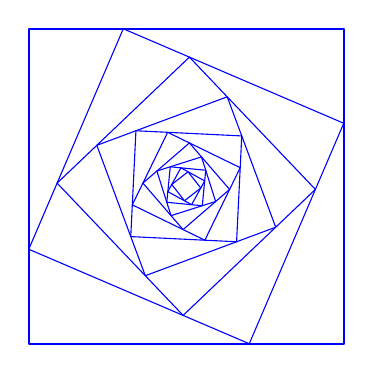
\begin{tikzpicture}[line cap=round, line join=round, thin, blue]
		\def\a{2}  %cạnh hình vuông
		\def\t{.7}  % tỷ lệ điểm cho vòng lặp tiếp
		\path 
		(-\a,-\a) coordinate (A1)
		(-\a,\a) coordinate (B1)
		(\a,\a) coordinate (C1)
		(\a,-\a) coordinate (D1);
		\draw[thick] (A1)--(B1)--(C1)--(D1)--cycle;
		\foreach \i[count=\j from 2] in {1,...,10}
		\draw
		(barycentric cs:A\i=\t,B\i=1-\t) coordinate (A\j)--
		(barycentric cs:B\i=\t,C\i=1-\t) coordinate (B\j)--
		(barycentric cs:C\i=\t,D\i=1-\t) coordinate (C\j)--
		(barycentric cs:D\i=\t,A\i=1-\t) coordinate (D\j)--cycle
		;
	\end{tikzpicture}
	}
	\shortans{$42{,}7$}
	\loigiai{
		Gọi hình vuông $C_1$ có cạnh $a_1=4$ và có diện tích là $S_1=a_1^2$.\\
		Cạnh của hình vuông $C_2$ là $a_2=\sqrt{{{\left( \dfrac{3}{4}{a_1} \right)}^2}+{{\left( \dfrac{1}{4}{a_1} \right)}^2}}=\dfrac{a_1\sqrt{10}}{4}$.\\
		Diện tích của hình vuông $C_2$ là $S_2=\dfrac{5}{8}{a_1}^2=\dfrac{5}{8}{S_1}$.\\
		Cạnh của hình vuông $C_3$ là $a_3=\sqrt{{{\left( \dfrac{3}{4}{a_2} \right)}^2}+{{\left( \dfrac{1}{4}{a_2} \right)}^2}}=\dfrac{a_2\sqrt{10}}{4}=a_1.{{\left( \dfrac{\sqrt{10}}{4} \right)}^2}$.\\
		Diện tích của hình vuông $C_3$ là $S_3={{\left( \dfrac{5}{8} \right)}^2}{a_1}^2={{\left( \dfrac{5}{8} \right)}^2}{S_1}$.\\
		Lý luận tương tự ta có dãy các hình vuông $C_1,\,C_2,\,C_3,\ldots,C_n,\ldots$ có các diện tích lần lượt là $S_1,\,S_2,\,S_3,\ldots,S_n,\ldots$ tạo thành một cấp số nhân lùi vô hạn với số hạng đầu là: $u_1=S_1=16$ và công bội $q=\dfrac{5}{8}$.\\
		Vậy tổng diện tích của các hình vuông là\\
		$S=S_1+\,S_2+\,S_3+\ldots+S_n+\ldots=\dfrac{u_1}{1-q}=\dfrac{16}{1-\tfrac{5}{8}}=\dfrac{128}{3}\approx 42{,}7$.}
\end{ex}
	\begin{ex}%[1D2V2-6]
		Tìm số hạng đầu tiên, công sai và tổng của $20$ số hạng đầu tiên của cấp số cộng $(u_n)$ biết rằng  $\heva{& {u_5}=19 \\
			& {u_9}=35}$.
		\shortans{$820$}
		\loigiai{
			Áp dụng công thức $u_n=u_1+(n-1)d$, ta có $\heva{ 
				& {u_5}=19 \\
				& {u_9}=35 } \Leftrightarrow \heva{ 
				& {u_1}+4d=19 \\
				& {u_1}+8d=35 }\Leftrightarrow \heva{ 
				& {u_1}=3 \\
				& d=4.}$\\
			Vậy số hạng đầu tiên $u_1=3$, công sai $d=4$.\\
			Tổng của $20$ số hạng đầu tiên: ${S_{20}}=\dfrac{20\left( 2u_1+19d \right)}{2}=10\left( 2\cdot3+19\cdot4 \right)=820$.}
	\end{ex}
	\begin{ex}%[1D1N6-8] 
		Hằng ngày mực nước tại một cảng biển lên xuống theo thuỷ triều. Độ sâu $h$ m của mực nước theo thời gian $t$ (giờ) trong một ngày được cho bởi công thức
		\centerline{$h=11+2\sin\left(\dfrac{\pi}{12}t\right) ~\text{với} ~0\leq t\leq 24$.}
		Tìm thời điểm mà mực nước tại cảng là cao nhất.
		\shortans[3]{$6$}
		\loigiai{
			Ta có
			\begin{eqnarray*}
				&&-1\le\sin\left(\dfrac{\pi}{12}t\right)\le 1\\
				&\Leftrightarrow & 11-2\le 11+2\sin\left(\dfrac{\pi}{12}t\right)\le 11+2\\
				&\Leftrightarrow& 9\le h\le 13
			\end{eqnarray*}
			Vậy mực nước tại cảng cao nhất bằng $13$ m khi
			\begin{eqnarray*}
				&&\sin\left(\dfrac{\pi}{12}t\right)=1\\
				&\Leftrightarrow & \left(\dfrac{\pi}{12}t\right)=\dfrac{\pi}{2}+2k\pi\\
				&\Leftrightarrow & t=6+24k ~\left(k\in\mathbb{Z}\right).
			\end{eqnarray*}
			Mà $0\le t\le 24$ nên $t=6$.\\ Vậy thời điểm mà mực nước tại cảng cao nhất là lúc $6$ (giờ).
		}
	\end{ex}
	\begin{ex}%[1D1V5-6]
			Một quả đạn pháo được bắn khỏi nòng pháo với vận tốc ban đầu $v_0$  m/s hợp với phương ngang một góc $\alpha $. Ta biết rằng, nếu bỏ qua sức cản của không khí và coi quả đạn pháo được bắn ra từ mặt đất thì quỹ đạo của quả đạn tuân theo phương trình $y=\dfrac{-g}{2v_0^2\cos^2\alpha }{x^2}+x\tan\alpha $, ở đó $g=9{,}8$ m/s$^2$ là gia tốc trọng trường. Biết quả đạn có tầm bắn xa nhất theo phương ngang $x_{\max}=9183{,}7$ (m), khi đó $v_0$ bằng bao nhiêu (kết quả làm tròn đến hàng đơn vị).
			\shortans{$300$}
			\loigiai{
				Chọn hệ trục tọa độ có gốc tọa độ đặt tại vị trí khẩu pháo, trục $Ox$ theo phương ngang và chiều dương trùng với hướng khẩu pháo.\\
				\begin{center}
				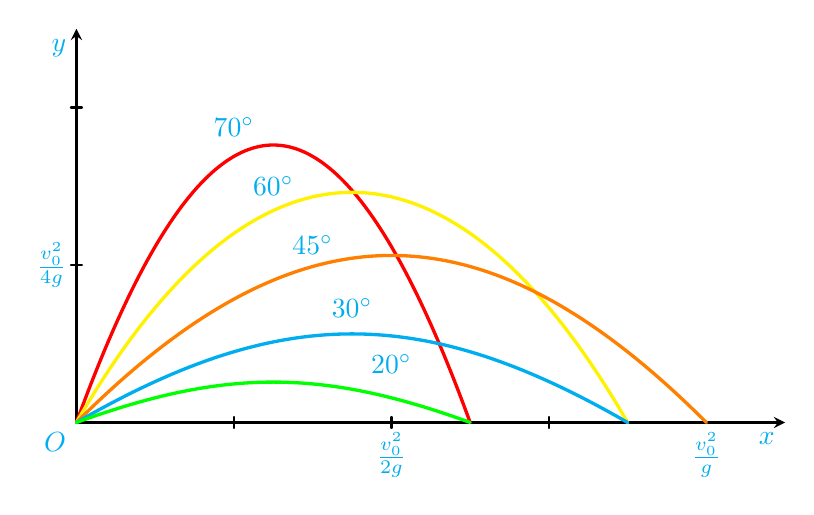
\begin{tikzpicture}[line join=round, line cap=round,>=stealth,thick]
					\draw[-stealth,thick] (0,0) -- (9,0) node[cyan,below left]{$x$};
					\draw[-stealth,thick] (0,0) -- (0,5) node[cyan,below left]{$y$};
					\foreach \x in {2,4,6}
					\draw [shift={(\x,0)}, color=black] (0pt,2pt)--(0pt,-2pt);
					\foreach \y in {2,4}
					\draw [shift={(0,\y)}, color=black] (2pt,0pt)--(-2pt,0pt);
					\draw[red,very thick] (0,0) .. controls +(70:5) and +(110:5) .. (5,0);
					\draw[yellow,very thick] (0,0) .. controls +(60:4.5) and +(120:4.5) .. (7,0);
					\draw[orange,very thick] (0,0) .. controls +(45:4) and +(135:4) .. (8,0);	
					\draw[cyan,very thick] (0,0) .. controls +(30:3) and +(150:3) .. (7,0);	
					\draw[green,very thick] (0,0) .. controls +(20:2) and +(160:2) .. (5,0);
					\draw[cyan] 
					(0,0) node[below left]{$O$}
					(0,2) node[left]{$\frac{v_{0}^{2}}{4g}$}
					(4,0) node[below]{$\frac{v_{0}^{2}}{2g}$}
					(8,0) node[below]{$\frac{v_{0}^{2}}{g}$}
					(2,4) node[below] {$70^\circ$}
					(2.5,3) node {$60^\circ$}
					(3,2) node[above] {$45^\circ$}
					(3.5,1.2) node[above] {$30^\circ$}
					(4,1) node[below] {$20^\circ$}
					;	
				\end{tikzpicture}
				\end{center}
				Ta biết rằng quỹ đạo của quả đạn pháo có dạng đường parabol có phương trình \\$y=\dfrac{-g}{2v_0^2\cdot \cos^2\alpha}{x^2}+x\cdot\tan\alpha $, ở đó $g=9{,}8$ m/s$^2$ là gia tốc trọng trường.\\
				Quả đạn chạm đất khi $y=0\Leftrightarrow \dfrac{-g}{2v_0^2\cos^2\alpha }{x^2}+x\tan\alpha =0$ $\Leftrightarrow$ 
				$\hoac{& x=0 \\
					& x=\dfrac{v_0^2\sin 2\alpha }{g}}$.\\
				Do đó quả đạn tiếp đất khi $x=\dfrac{v_0^2\sin 2\alpha }{g}$.\\
				Ta có $x=\dfrac{v_0^2\sin 2\alpha }{g}\le \dfrac{v_0^2}{g}$, đẳng thức xảy ra khi $\sin 2\alpha =1$ hay $\alpha =45{}^\circ $.\\
				Suy ra quả đạn có tầm bắn xa nhất theo phương ngang là ${x_{\max }}=\dfrac{v_0^2}{g}=9183{,}7$.\\
				$v_0^2 = 9183{,}7\cdot 9{,}8 = 90000{,}26$.\\
			Do đó	$v_0\approx 300$ (m/s).
			}
		\end{ex}
	\begin{ex}%[1H4H2-1]
		Cho tứ diện $ABCD$. Điểm $I$ và $J$ theo thứ tự là trung điểm của $AD$ và $AC$, $G$ là trọng tâm tam giác $BCD$. Giao tuyến của hai mặt phẳng $(GIJ)$ và $(BCD)$ cắt $BD$ tại $E$, cắt $BC$ tại $F$. Tính tỉ số $\dfrac{EF}{IJ}$ (kết quả làm tròn đến hàng phần trăm).
		\shortans{$0{,}67$}
		\loigiai{
				\begin{center}
			\begin{tikzpicture}[scale=0.7, font=\footnotesize,line join=round, line cap=round, >=stealth]
				\path
				(0,0) coordinate (B)
				++(-45:3) coordinate (C)
				($(B)+(5,0)$) coordinate (D)
				($(B)+(1,4)$) coordinate (A)
				($(A)!0.5!(C)$) coordinate (J)
				($(A)!0.5!(D)$) coordinate (I)
				($(B)!2/3!(C)$) coordinate (F)
				($(B)!2/3!(D)$) coordinate (E)
				($(E)!0.5!(F)$) coordinate (G)
				($(C)!0.5!(D)$) coordinate (K)
				($(E)!1.5!(F)$) coordinate (X) node[above] {$x$}
				;
				\foreach \i in {B,C,D}{\draw (A)--(\i);}
				\draw
				(B)--(C)--(D)
				(X)--(F)--(J)--(I)
				;
				\draw[dashed,thin]
				(B)--(D)
				(F)--(E)--(I)
				(J)--(G)--(I)
				(B)--(K)
				;
				\foreach \i/\g in {A/90,B/180,C/-90,D/0,I/30,J/-150,E/45,F/-90, G/-90, K/-30}
				\fill[black] (\i) circle(1pt)+(\g:4mm)node[scale=1]{$\i$};
			\end{tikzpicture}
		\end{center}
				$IJ$ là đường trung bình của $\triangle ACD$ nên $IJ \parallel CD$ và $IJ = \dfrac{1}{2} CD.\quad (1)$\\
				Ta có $\heva{&IJ \parallel CD \\ &IJ \subset(GIJ) \\ &CD \subset(BCD) \\ &G \in(IJG) \cap(BCD)} \Rightarrow \heva{&G x=(GIJ) \cap (BCD) \\ &Gx \parallel IJ \parallel CD.}$\\
				Suy ra giao tuyến $Gx \equiv EF$.\\
				Tứ giác $IJFE$ có $IJ \parallel FE$ nên là hình thang.\\
				Vì $G$ là trọng tâm $\triangle BCD$ và $EF \parallel CD$.\\
				Nên $\dfrac{EF}{CD} = \dfrac{BE}{BD} = \dfrac{BG}{BK} = \dfrac{1}{3}. \quad (2)$\\
				Từ $(1)$ và $(2)$, suy ra $\dfrac{EF}{IJ} = \dfrac{\dfrac{2}{3}}{\dfrac{1}{2}} = \dfrac{2}{3}\approx 0{,}67$.	
		}
	\end{ex}
\Closesolutionfile{ans}
\indapan{6}{ans/ans-CTST_1-OTGK1_De3-KQ}